\section{Installazione manuale}\label{sec:openstack_manual_installation}
In questa sezione verrà effettuato il deploy del cloud OpenStack installando un charm alla volta.
% 
Tuttavia, Juju si occuperà dell'installazione ed effettiva configurazione di ogni singolo componente.
% 
L'intero processo di installazione richiede non poco tempo, e a seconda della velocità delle macchine e del tempo impiegato dall'operatore possono occorrere all'incirca 30/60 minuti per un'installazione veloce fino a 120/180 minuti per un'installazione più analitica.
% 
Per maggiori dettagli, si rimanda alla documentazione \cite{openstack_installation_juju}.

Come prima cosa, bisogna assicurarsi che i comandi verranno impartiti al Juju controller e al model corretto (\cref{sec:juju_model_create}).
% 
Per farlo, baserà eseguire il comando mostrato nel \cref{lst:openstack_install_switch}.

% \begin{minipage}{0.96\linewidth} 
\begin{lstlisting}[
    language=mybash, 
    caption={Comando per selezionare il Juju controller e il corretto model.}, 
    label={lst:openstack_install_switch},
]
juju switch maas-controller:openstack
\end{lstlisting}
% \end{minipage}

\bigskip\noindent
Ora è possibile effettuare i deploy dei vari charm;
% 
tra l'esecuzione di un comando e l'altro non è necessario aspettare che Juju finisca nei vari procedimenti.
% 
Tuttavia, specialmente le prime volte, è consigliato eseguire un comando alla volta per apprendere al meglio le varie fasi di deploy.



 \bigskip\noindent
% \hfill\break
\paragraph{Ceph OSD.}
Il primo charm che si andrà ad installare è quello inerente al gestore d'archiviazione dei dati, ceph-osd (\cref{sec:ceph}).
% 
Questo charm bisogna configurarlo il maniera corretta, indicandogli dispositivi di storage da utilizzare.
% 
in questo progetto tutti i nodi montano gli stessi dispositivi di storage.

Per configurare i charm in maniera agile, si utilizzano i file di configurazione \code{YAML};
% 
quindi è stato creato il file \code{ceph-osd.yaml} con le configurazioni mostrate nel \cref{lst:openstack_install_ceph-osd.yaml}.

% \begin{minipage}{0.96\linewidth} 
\begin{lstlisting}[
    language=yaml, 
    caption={Configurazione di \emph{ceph-osd} nel file \emph{ceph-sod.yaml}.}, 
    label={lst:openstack_install_ceph-osd.yaml},
]
ceph-osd:
  osd-devices: /dev/sda /dev/sdb
  source: distro
\end{lstlisting}
% \end{minipage}

\bigskip\noindent
Il charm ceph-osd verrà installato su tutti e 4 i nodi;
% 
essendo il primo deploy, sui nodi non è ancora presente il sistema operativo, quindi durante questa fase verrà installato anche quest'ultimo in maniera automatica, applicando le immagini scaricate attraverso MAAS.
% 
nel \cref{lst:openstack_install_ceph-osd} viene mostrato il comando per il deploy di ceph-osd.
% \begin{minipage}{0.96\linewidth} 
\begin{lstlisting}[
    language=mybash, 
    caption={Deploy del charm \emph{ceph-osd}.}, 
    label={lst:openstack_install_ceph-osd},
]
juju deploy -n 4 --series jammy --channel quincy/stable --config ceph-osd.yaml --constraints tags=compute ceph-osd
\end{lstlisting}
% \end{minipage}
\begin{itemize}
    \item Con \code{-n} viene indicato su quanti nodi effettuare il deploy del charm, in questo caso su tutti e quattro i nodi.
    
    \item Con \code{-{}-series} e con \code{-{}-channel} viene indicato di fatto la versione del sistema operativo e del charm.

    \item Con \code{-{}-config} è possibile specificare il file \code{YAML} per applicare delle configurazioni personalizzate.

    \item  Con \code{-{}-constraints} è possibile specificare in maniera accurata i requisiti  hardware per le nuove macchine su cui effettuare il deploy.
    % 
    Questi requisiti possono essere ad esempio memoria ram, tag, space, etc.
    % 
    In questo caso specifico è stato indicato di effettuare il deploy su tutti i nodi aventi il tag \emph{compute} (impostato durante le fasi di add dei nodi su MAAS nella \cref{itm:tag_node} della \cref{subsubsec:maas_add_node}).
\end{itemize}



% \bigskip
\paragraph{Nova Compute.}
Il prossimo charm da installare è nova-compute (\cref{sec:openstack_nova}), usato per gestire le macchine virtuali.
% 
Anche in questo caso l'installazione del charm sarà personalizzata con l'inserimento di qualche impostazione salvata nel file \code{nova-compute.yaml}, contenente le configurazioni mostrate nel \cref{lst:openstack_install_nova-compute.yaml}.
% \begin{minipage}{0.96\linewidth} 
\begin{lstlisting}[
    language=yaml, 
   caption={Configurazione di \emph{nova-compute} nel file \emph{nova-compute.yaml}.},
    label={lst:openstack_install_nova-compute.yaml},
]
nova-compute:
  config-flags: default_ephemeral_format=ext4
  enable-live-migration: true
  enable-resize: true
  migration-auth-type: ssh
  virt-type: qemu
  openstack-origin: distro
\end{lstlisting}
% \end{minipage}

\bigskip\noindent
Quindi è possibile effettuare il deploy del charm nova-compute su tre macchine.
% \begin{minipage}{0.96\linewidth} 
\begin{lstlisting}[
    language=mybash, 
   caption={Deploy del charm \emph{nova-compute}.},
    label={lst:openstack_install_nova-compute},
]
juju deploy -n 3 --to 1,2,3 --series jammy --channel yoga/stable --config nova-compute.yaml nova-compute
\end{lstlisting}
% \end{minipage}
\begin{itemize}
    \item Con \code{-{}-to} è possibile indicare in maniera precisa su quali macchine andare ad effettuare i deploy del charm.
    % 
    Queste macchine devono essere già state aggiunte in Juju, e in questo caso è avvenuto con il primo comando di deploy.
    % 
    Il numero indicato rappresenta l'indice della macchina, ed è possibile prenderne nota attraverso il comando \code{juju status}.   
\end{itemize}


% \bigskip
\paragraph{MySQL InnoDB Cluster.}
Il charm che si occuperà della creazione e gestione del database per archiviare tutte le varie informazioni che gli altri charm utilizzeranno è mysql-innodb-cluster.
% 
Questo charm richiede sempre almeno tre unit, e saranno containerizzate tramite LXD nelle macchine 0, 1 e 2.
% \begin{minipage}{0.96\linewidth} 
\begin{lstlisting}[
    language=mybash, 
   caption={Deploy del charm \emph{mysq-innodb-cluster}.},
    label={lst:openstack_install_mysq-innodb-cluster},
]
juju deploy -n 3 --to lxd:0,lxd:1,lxd:2 --series jammy --channel 8.0/stable mysql-innodb-cluster
\end{lstlisting}
% \end{minipage}



% \bigskip
\paragraph{Vault.}
In questa fase verrà installato il charm vault (\cref{sec:vault}) in una unica unit, il quale gestirà tutte quelle informazioni sensibili denominate come \emph{secret}, come ad esempio i certificati TLS per la comunicazione crittografata tra le applicazioni cloud.
% \begin{minipage}{0.96\linewidth} 
\begin{lstlisting}[
    language=mybash, 
   caption={Deploy del charm \emph{vault}.},
    label={lst:openstack_install_vault},
]
juju deploy --to lxd:3 --series jammy --channel 1.7/stable vault
\end{lstlisting}
% \end{minipage}

\bigskip\noindent
Questo charm deve essere messa in relazione con il database del cloud.
% 
Per farlo, è necessario installare una unit specifica del subordinate \emph{mysql-router}, che si comporterà da tramite tra vault e mysql-innodb-cluster.
% 
Una volta installato, è possibile aggiungere le relazioni come mostrato in \cref{lst:openstack_install_vault_rel}.
% \begin{minipage}{0.96\linewidth} 
\begin{lstlisting}[
    language=mybash, 
   caption={Deploy del subordinate \emph{mysql-router} per le relazioni con vault.},
    label={lst:openstack_install_vault_rel},
]
juju deploy --channel 8.0/stable mysql-router vault-mysql-router
juju add-relation vault-mysql-router:db-router mysql-innodb-cluster:db-router
juju add-relation vault-mysql-router:shared-db vault:shared-db
\end{lstlisting}
% \end{minipage}


\subparagraph{Configurazione di vault.}\label{subpar:vault_configuration}
Finita l'installazione di vault, è necessario inizializzarlo e "aprirlo".
% 
Innanzitutto bisogna installare il client Vault attraverso snap.
% \begin{minipage}{0.96\linewidth} 
\begin{lstlisting}[
    language=mybash, 
   caption={Installazione del client \emph{Vault}.},
    label={lst:openstack_install_vault_install},
]
sudo snap install vault
\end{lstlisting}
% \end{minipage}

\bigskip\noindent
Successivamente, si estrapola l'indirizzo IP del container sul quale è stato installato; 
% 
l'indirizzo IP è possibile visionarlo anche attraverso \code{juju status}.
% 
L'indirizzo IP serve per inizializzare la variabile \code{VAULT\_ADDR} con l'URI del charm vault, necessaria per le fasi successive.
% \begin{minipage}{0.96\linewidth} 
\begin{lstlisting}[
    language=mybash, 
   caption={Crezione della variabile d'ambiente \code{VAULT\_ADDR}.},
    label={lst:openstack_install_vault-ip},
]
IP_VAULT=$(juju status --format=yaml vault | grep public-address | awk '{print $2}' | head -1)
export VAULT_ADDR="http://${IP_VAULT}:8200"
\end{lstlisting}
% \end{minipage}

\bigskip\noindent
A questo punto è possibile inizializzare Vault, indicandogli di creare cinque chiavi e di necessitarne tre per la sua apertura.
% 
Queste chiavi poi sono state esportate sul file \code{vault-keys} per una miglior comprensione ed utilizzo.
% 
Queste chiavi sono salvate in chiaro, ed è consigliato conservarle in un luogo sicuro.
% \begin{minipage}{0.96\linewidth} 
\begin{lstlisting}[
    language=mybash, 
   caption={Generazione delle chiavi d'apertua del vault.},
    label={lst:openstack_install_vault_keygen},
]
vault operator init -key-shares=5 -key-threshold=3 > vault-keys
\end{lstlisting}
% \end{minipage}

\bigskip\noindent
Ora è possibile aprire Vault, utilizzando tre delle cinque chiavi generate nel \cref{lst:openstack_install_vault_keygen}.
% \begin{minipage}{0.96\linewidth} 
\begin{lstlisting}[
    language=mybash, 
   caption={Unseal del client Vault.},
    label={lst:openstack_install_vault_unseal},
]
vault operator unseal <key1>
vault operator unseal <key2>
vault operator unseal <key3>
\end{lstlisting}
% \end{minipage}
\begin{itemize}
    \item Al posto di \code{<key1>}, \code{<key2>} e \code{<key3>}, bisogna inserire tre chiavi a piacere tra le cinque a disposizione. 
\end{itemize}

\bigskip\noindent
Una volta aperto il client Vault, bisogna autorizzare il charm vault a poter interagire con esso e creare e gestire i secret.
% 
Per farlo, viene creato un token root dalla durata di 10 minuti.
% \begin{minipage}{0.96\linewidth} 
\begin{lstlisting}[
    language=mybash, 
   caption={Generazione del token temporaneo.},
    label={lst:openstack_install_vault_tokengen},
]
export VAULT_TOKEN=<Initial Root Token>
vault token create -ttl=10m
\end{lstlisting}
% \end{minipage}
\begin{itemize}
    \item Il \code{<Initial Root Token>} è possibile trovarlo nell'output (nel file se è stato salvato) del \cref{lst:openstack_install_vault_keygen}.
\end{itemize}

\bigskip\noindent
Infine, è possibile autorizzare il charm vault con il token appena generato nel \cref{lst:openstack_install_vault_tokengen}.
% 
Con il comando \code{run-action}, è possibile far eseguire ai charm un'azione tra quelle che concedono, in base all'implementazione del charm stesso.
% \begin{minipage}{0.96\linewidth} 
\begin{lstlisting}[
    language=mybash, 
   caption={Autorizzazione al charm \emph{vault}.},
    label={lst:openstack_install_vault_authorise},
]
juju run-action --wait vault/leader authorize-charm token=<token>
\end{lstlisting}
% \end{minipage}
\begin{itemize}
    \item Al posto di \code{<token>} bisogna inserire il token temporaneo generato nel \cref{lst:openstack_install_vault_tokengen}.
\end{itemize}


\bigskip\noindent
A charm autorizzato, è possibile creare un certificato autofirmato se non se ne possiede uno rilasciato da una CA.
% \begin{minipage}{0.96\linewidth} 
\begin{lstlisting}[
    language=mybash, 
   caption={Creazione del certificato autofirmato.},
    label={lst:openstack_install_vault_self-crt},
]
juju run-action --wait vault/leader generate-root-ca > vault-ca.crt
\end{lstlisting}
% \end{minipage}


\bigskip\noindent
Come ultimo passaggio, verrà collegato il certificato di vault, creato nel \cref{lst:openstack_install_vault_self-crt}, al DB del cloud attraverso l'aggiunta della relativa relazione.
% \begin{minipage}{0.96\linewidth} 
\begin{lstlisting}[
    language=mybash, 
   caption={Aggiunta della relazione per collegare il certificato a DB.},
    label={lst:openstack_install_vault_add_crt},
]
juju add-relation mysql-innodb-cluster:certificates vault:certificates
\end{lstlisting}
% \end{minipage}



\paragraph{Neutron.}
Per implementare la rete con Neutron (\cref{sec:openstack_neutron}), verranno installati quattro charms:
% 
\begin{itemize}
    \item ovn-central per il controllo delle OVN (\cref{subsubsec:ovs}), installato su tre unit.
    \item neutron-api fornisce il servizio di API di Neutron, installato in una unica unit.
    \item neutron-api-plugin-ovn subordinate di neutron-api.
    \item ovn-chassis subordinate di ovn-central.
\end{itemize}
% 
Nel file \code{neutron.yaml} verranno inserite le configurazioni della rete che Neutron utilizzerà.
% \begin{minipage}{0.96\linewidth} 
\begin{lstlisting}[
    language=yaml, 
   caption={Configurazione di \emph{Neutron} nel file \emph{neutron.yaml}.},
    label={lst:openstack_install_neutron.yaml},
]
ovn-chassis:
  bridge-interface-mappings: br-ex:enp3s0
  ovn-bridge-mappings: physnet1:br-ex
neutron-api:
  neutron-security-groups: true
  flat-network-providers: physnet1
  openstack-origin: distro
ovn-central:
  source: distro
\end{lstlisting}
% \end{minipage}
\begin{itemize}
    \item \code{bridge-interface-mappings} indica la mappatura del \emph{OvS bridge} creato nel \cref{itm:maas_ovs_bridge} nella \cref{subsubsec:maas_add_node} ed è composto dal \emph{bridge name}  seguito dai due punti e dal nome dell'interfaccia di rete.
    % 
    In questo caso, il \emph{bridge name} dato è stato \code{br}, mentre le interfacce di rete erano nominate come \code{enp3s0}.
    
    \item \code{physnet1} è il nome che viene associato al provider di rete di tipo flat.
\end{itemize}



\bigskip\noindent
Quindi, si procede con il deploy dei quattro charm.
% \begin{minipage}{0.96\linewidth} 
\begin{lstlisting}[
    language=mybash, 
   caption={Deploy dei quattro charm che comporranno \emph{Neutron}.},
    label={lst:openstack_install_neutron},
]
juju deploy -n 3 --to lxd:0,lxd:1,lxd:2 --series jammy --channel 22.03/stable --config neutron.yaml ovn-central
juju deploy --to lxd:1 --series jammy --channel yoga/stable --config neutron.yaml neutron-api
juju deploy --channel yoga/stable neutron-api-plugin-ovn
juju deploy --channel 22.03/stable --config neutron.yaml ovn-chassis
\end{lstlisting}
% \end{minipage}

\bigskip\noindent
Dopo il deploy, è possibile aggiungere le relazioni che i charm necessitano.
% 
Anche in questo caso viene installata una unit per il collegamento di Neutron con il DB (come nel \cref{lst:openstack_install_vault_rel})
% \begin{minipage}{0.96\linewidth} 
\begin{lstlisting}[
    language=mybash, 
   caption={Aggiunta delle varie relazioni per \emph{Neutron}.},
    label={lst:openstack_install_neutron_rel},
]
juju add-relation neutron-api-plugin-ovn:neutron-plugin neutron-api:neutron-plugin-api-subordinate
juju add-relation neutron-api-plugin-ovn:ovsdb-cms ovn-central:ovsdb-cms
juju add-relation ovn-chassis:ovsdb ovn-central:ovsdb
juju add-relation ovn-chassis:nova-compute nova-compute:neutron-plugin
juju add-relation neutron-api:certificates vault:certificates
juju add-relation neutron-api-plugin-ovn:certificates vault:certificates
juju add-relation ovn-central:certificates vault:certificates
juju add-relation ovn-chassis:certificates vault:certificates

juju deploy --channel 8.0/stable mysql-router neutron-api-mysql-router
juju add-relation neutron-api-mysql-router:db-router mysql-innodb-cluster:db-router
juju add-relation neutron-api-mysql-router:shared-db neutron-api:shared-db
\end{lstlisting}
% \end{minipage}



% \bigskip
\paragraph{Keystone.}
Il charm keystone (\cref{sec:openstack_keystone}) è il componente che si occuperà di fornire le API per l'autenticazione dei client.
% 
Verrà installato in un'unica unit.
% 
% Nel \cref{lst:openstack_install_keystone} viene 
% \begin{minipage}{0.96\linewidth} 
\begin{lstlisting}[
    language=mybash, 
   caption={Deploy del charm \emph{keystone}.},
    label={lst:openstack_install_keystone},
]
juju deploy --to lxd:0 --series jammy --channel yoga/stable keystone

juju deploy --channel 8.0/stable mysql-router keystone-mysql-router
juju add-relation keystone-mysql-router:db-router mysql-innodb-cluster:db-router
juju add-relation keystone-mysql-router:shared-db keystone:shared-db

juju add-relation keystone:identity-service neutron-api:identity-service
juju add-relation keystone:certificates vault:certificates
\end{lstlisting}
% \end{minipage}



% \bigskip
\paragraph{RabbitMQ.}
RabbitMQ è il servizio che implementa il broker per il protocollo di messaggistica AMQP e il suo charm rabbitmq-server viene installato su un'unica unit.
% \begin{minipage}{0.96\linewidth} 
\begin{lstlisting}[
    language=mybash, 
   caption={Deploy del charm \emph{rabbitmq-server}.},
    label={lst:openstack_install_rabbitmq},
]
juju deploy --to lxd:2 --series jammy --channel 3.9/stable rabbitmq-server
juju add-relation rabbitmq-server:amqp neutron-api:amqp
juju add-relation rabbitmq-server:amqp nova-compute:amqp
\end{lstlisting}
% \end{minipage}



% \bigskip
\paragraph{Nova cloud controller.}
Questa applicazione implementa per conto di Nova tre servizi: uno inerente alle API, uno per il coordinamento e supporto per le query del DB con Nova ed infine uno per la selezione dei nodi durante la creazione di istanze delle macchine virtuali.
% 
Anche in questo caso è necessario aggiungere delle configurazioni attraverso il file dedicato \code{ncc.yaml}.
% \begin{minipage}{0.96\linewidth} 
\begin{lstlisting}[
    language=yaml, 
   caption={Configurazione di \emph{Nova Cloud Controller} nel file \emph{ncc.yaml}.},
    label={lst:openstack_install_ncc.yaml},
]
nova-cloud-controller:
  network-manager: Neutron
  openstack-origin: distro
\end{lstlisting}
% \end{minipage}

\noindent
Dopodiché è possibile installare il charm nova-cloud-controller su un'unica istanza, con annesso subordinate per il collegamento con il database.
% \begin{minipage}{0.96\linewidth} 
\begin{lstlisting}[
    language=mybash, 
   caption={Deploy del charm \emph{nova-cloud-controller}.},
    label={lst:openstack_install_nova-cloud-controller},
]
juju deploy --to lxd:3 --series jammy --channel yoga/stable --config ncc.yaml nova-cloud-controller

juju deploy --channel 8.0/stable mysql-router ncc-mysql-router
juju add-relation ncc-mysql-router:db-router mysql-innodb-cluster:db-router
juju add-relation ncc-mysql-router:shared-db nova-cloud-controller:shared-db

juju add-relation nova-cloud-controller:identity-service keystone:identity-service
juju add-relation nova-cloud-controller:amqp rabbitmq-server:amqp
juju add-relation nova-cloud-controller:neutron-api neutron-api:neutron-api
juju add-relation nova-cloud-controller:cloud-compute nova-compute:cloud-compute
juju add-relation nova-cloud-controller:certificates vault:certificates
\end{lstlisting}
% \end{minipage}



% \bigskip
\paragraph{Placement.}
Placement (\cref{sec:openstack_placement}), attraverso il charm placement, si occuperà di inventariare le risorse del cloud e viene installato su un'unica unit.
% 
Anch'esso utilizza un subordinate per l'interfacciamento con il database.
% \begin{minipage}{0.96\linewidth} 
\begin{lstlisting}[
    language=mybash, 
   caption={Deploy del charm \emph{placement}.},
    label={lst:openstack_install_placement},
]
juju deploy --to lxd:3 --series jammy --channel yoga/stable placement

juju deploy --channel 8.0/stable mysql-router placement-mysql-router
juju add-relation placement-mysql-router:db-router mysql-innodb-cluster:db-router
juju add-relation placement-mysql-router:shared-db placement:shared-db

juju add-relation placement:identity-service keystone:identity-service
juju add-relation placement:placement nova-cloud-controller:placement
juju add-relation placement:certificates vault:certificates
\end{lstlisting}
% \end{minipage}



% \bigskip
\paragraph{OpenStack dashboard.}
La dashboard e la relativa interfaccia grafica via web dell'intero cloud OpenStack è implementata dall'applicazione Horizon (\cref{sec:openstack_horizon}), installato attraverso il charm openstack-dashboard in un'unica unit e il subordinate per la connessione con il database.
% \begin{minipage}{0.96\linewidth} 
\begin{lstlisting}[
    language=mybash, 
   caption={Deploy del charm \emph{openstack-dashboard}.},
    label={lst:openstack_install_openstack-dashboard},
]
juju deploy --to lxd:2 --series jammy --channel yoga/stable openstack-dashboard

juju deploy --channel 8.0/stable mysql-router dashboard-mysql-router
juju add-relation dashboard-mysql-router:db-router mysql-innodb-cluster:db-router
juju add-relation dashboard-mysql-router:shared-db openstack-dashboard:shared-db

juju add-relation openstack-dashboard:identity-service keystone:identity-service
juju add-relation openstack-dashboard:certificates vault:certificates
\end{lstlisting}
% \end{minipage}



% \bigskip
\paragraph{Glance.}
Glance (\cref{sec:openstack_glance}) è il servizio di OpenStack avente il compito della gestione delle immagini per le macchine virtuali.
% 
Viene implementato attraverso il charm glance su un'unica istanza con il relativo subordinate per la comunicazione con il DB.
% \begin{minipage}{0.96\linewidth} 
\begin{lstlisting}[
    language=mybash, 
   caption={Deploy del charm \emph{glance}.},
    label={lst:openstack_install_glance},
]
juju deploy --to lxd:3 --series jammy --channel yoga/stable glance

juju deploy --channel 8.0/stable mysql-router glance-mysql-router
juju add-relation glance-mysql-router:db-router mysql-innodb-cluster:db-router
juju add-relation glance-mysql-router:shared-db glance:shared-db

juju add-relation glance:image-service nova-cloud-controller:image-service
juju add-relation glance:image-service nova-compute:image-service
juju add-relation glance:identity-service keystone:identity-service
juju add-relation glance:certificates vault:certificates
\end{lstlisting}
% \end{minipage}



% \bigskip
\paragraph{Ceph (monitor).}
Il charm ceph-mon implementa il monitor per Ceph, ovvero quel componente che mantiene una copia della mappa dell'intero cluster.
% 
Anche questo viene configurato attraverso un file esterno, \code{ceph-mon.yaml}
% \begin{minipage}{0.96\linewidth} 
\begin{lstlisting}[
    language=yaml, 
   caption={Configurazione di \emph{Ceph Mon} nel file \emph{ceph-mon.yaml}.},
    label={lst:openstack_install_ceph-mon.yaml},
]
ceph-mon:
  expected-osd-count: 4
  monitor-count: 3
  source: distro
\end{lstlisting}
% \end{minipage}

\bigskip\noindent
Infine, viene installato su tre nodi.
% \begin{minipage}{0.96\linewidth} 
\begin{lstlisting}[
    language=mybash, 
   caption={Deploy del charm \emph{ceph-mon}.},
    label={lst:openstack_install_ceph-mon},
]
juju deploy -n 3 --to lxd:0,lxd:1,lxd:2 --series jammy --channel quincy/stable --config ceph-mon.yaml ceph-mon

juju add-relation ceph-mon:osd ceph-osd:mon
juju add-relation ceph-mon:client nova-compute:ceph
juju add-relation ceph-mon:client glance:ceph
\end{lstlisting}
% \end{minipage}
% juju config nova-compute libvirt-image-backend=rbd NON MESSO ???



% \bigskip
\paragraph{Cinder.}
Cinder (\cref{sec:openstack_cinder}) è l'ultimo componente che verrà configurato attraverso un file, \code{cinder.yaml}, per l'implementazione del servizio di block storage attraverso il charm cinder.
% \begin{minipage}{0.96\linewidth} 
\begin{lstlisting}[
    language=yaml, 
   caption={Configurazione di \emph{Cinder} nel file \emph{cinder.yaml}.},
    label={lst:openstack_install_cinder.yaml},
]
cinder:
  block-device: None
  glance-api-version: 2
  openstack-origin: distro
\end{lstlisting}
% \end{minipage}

\bigskip\noindent
Quindi si installa il charm cinder, il subordinate per la comunicazione con il database e l'aggiunta delle relative relazioni.
% \begin{minipage}{0.96\linewidth} 
\begin{lstlisting}[
    language=mybash, 
   caption={Deploy del charm \emph{cinder}.},
    label={lst:openstack_install_cinder},
]
juju deploy --to lxd:1 --series jammy --channel yoga/stable --config cinder.yaml cinder

juju deploy --channel 8.0/stable mysql-router cinder-mysql-router
juju add-relation cinder-mysql-router:db-router mysql-innodb-cluster:db-router
juju add-relation cinder-mysql-router:shared-db cinder:shared-db

juju add-relation cinder:cinder-volume-service nova-cloud-controller:cinder-volume-service
juju add-relation cinder:identity-service keystone:identity-service
juju add-relation cinder:amqp rabbitmq-server:amqp
juju add-relation cinder:image-service glance:image-service
juju add-relation cinder:certificates vault:certificates
\end{lstlisting}
% \end{minipage}

\bigskip\noindent
Infine, cinder necessita del subordinate cinder-ceph per poter interfacciarsi con Ceph;
% 
Infatti, sfrutta quest'ultimo come effettivo storage, limitandosi a fornire una virtualizzazione di essi.
% 
Nel \cref{lst:openstack_install_cinder.yaml} è possibile notare che attraverso l'opzione \code{block-device: None} non gli sono stati indicati i block device. 
% \begin{minipage}{0.96\linewidth} 
\begin{lstlisting}[
    language=mybash, 
   caption={Deploy del charm \emph{cinder-ceph}.},
    label={lst:openstack_install_cinder-ceph},
]
juju deploy --channel yoga/stable cinder-ceph
juju add-relation cinder-ceph:storage-backend cinder:storage-backend
juju add-relation cinder-ceph:ceph ceph-mon:client
juju add-relation cinder-ceph:ceph-access nova-compute:ceph-access
\end{lstlisting}
% \end{minipage}



% \bigskip
\paragraph{Ceph RADOS Gateway.}
L'ultimo componente che viene installato è Ceph RADOS Gateway, che attraveso il charm ceph-radosgw offre un gateway HTTP compatibile con S3 e Swift.
% 
Quest'ultimo charm viene installato su un'unica istanza.
% \begin{minipage}{0.96\linewidth} 
\begin{lstlisting}[
    language=mybash, 
   caption={Deploy del charm \emph{ceph-radosgw}.},
    label={lst:openstack_install_ceph-radosgw},
]
juju deploy --to lxd:0 --series jammy --channel quincy/stable ceph-radosgw
juju add-relation ceph-radosgw:mon ceph-mon:radosgw
\end{lstlisting}
% \end{minipage}


% \bigskip
\paragraph{Risultati finali.}
Dopo aver effettuato l'ultimo deploy, è necessario attendere che Juju porti a termine le varie operazioni.
% 
Una volta stabilizzato, l'output del comando \code{juju status} dovrebbe essere simile a come mostrato nelle \cref{fig:juju_status_finish_app,fig:juju_status_finish_unit,fig:juju_status_finish_machine}.
%
Tutte le applicazioni e le unit avranno lo status \emph{active} con i relativi agent in \emph{idle}, e come message mostreranno che sono in \emph{ready}.

% \begin{figure}%[H]
%     \centering
%     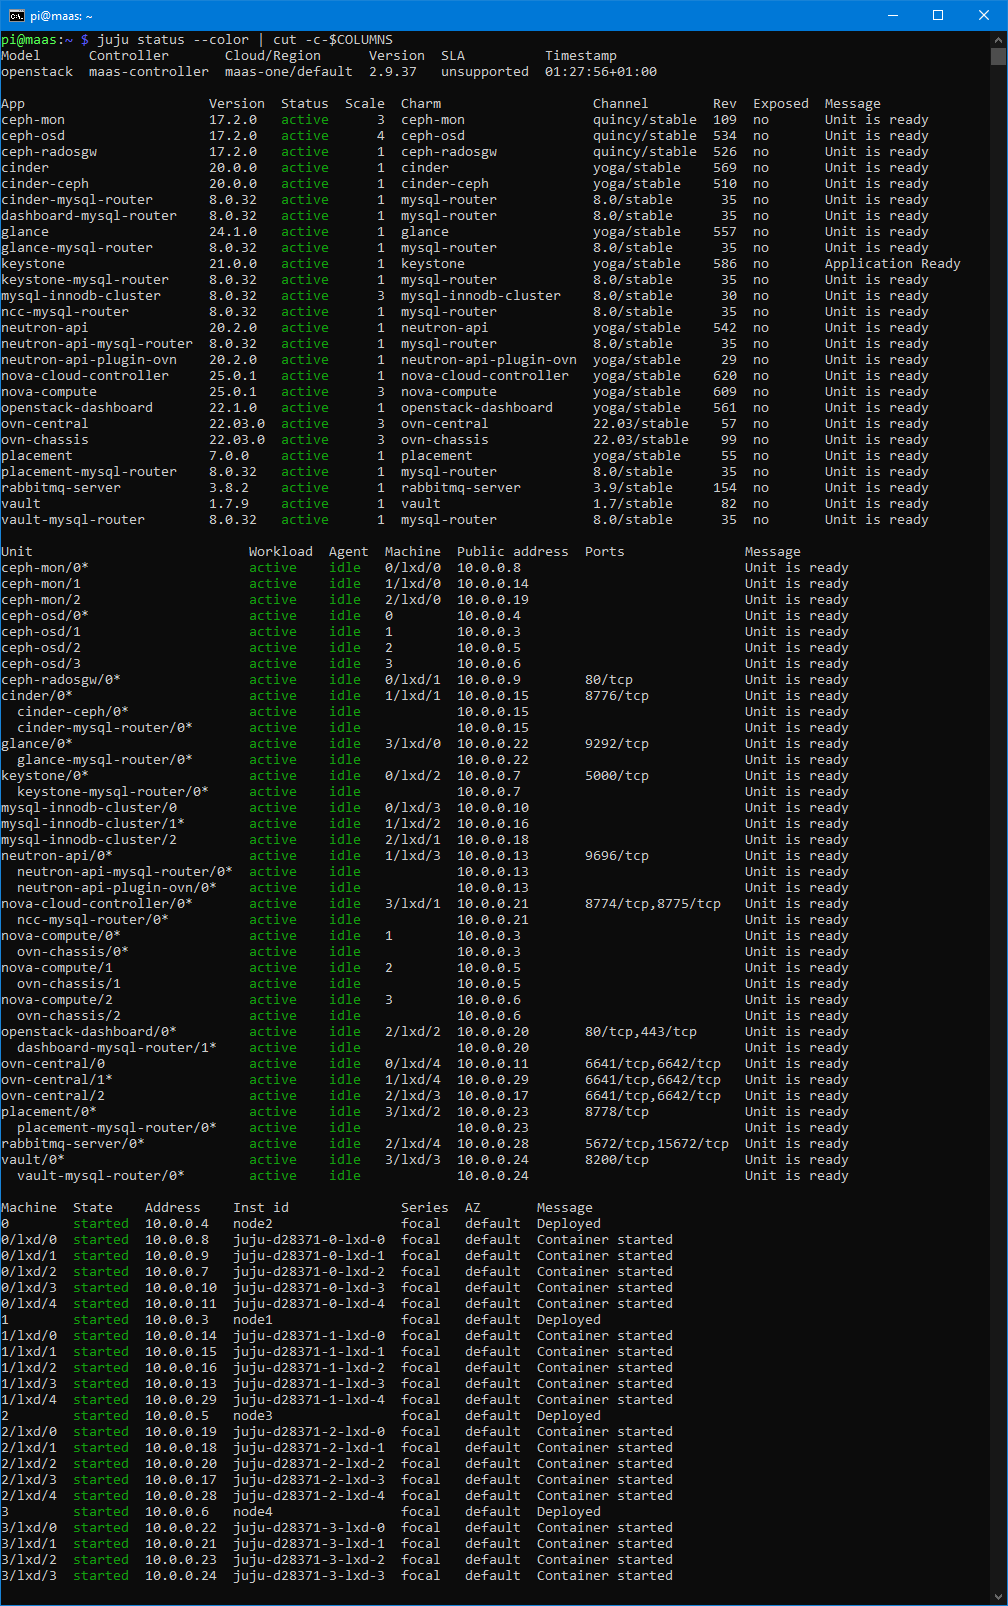
\includegraphics[width=1\linewidth]{tesi/files/immagini/openstack/finish.png}
%     \vspace*{-8mm}
%     \caption{Status finale del cloud OpenStack post deployment con i charm.}
%     \label{fig:juju_status_finish}
% \end{figure}

\begin{figure}%[H]
    \centering
    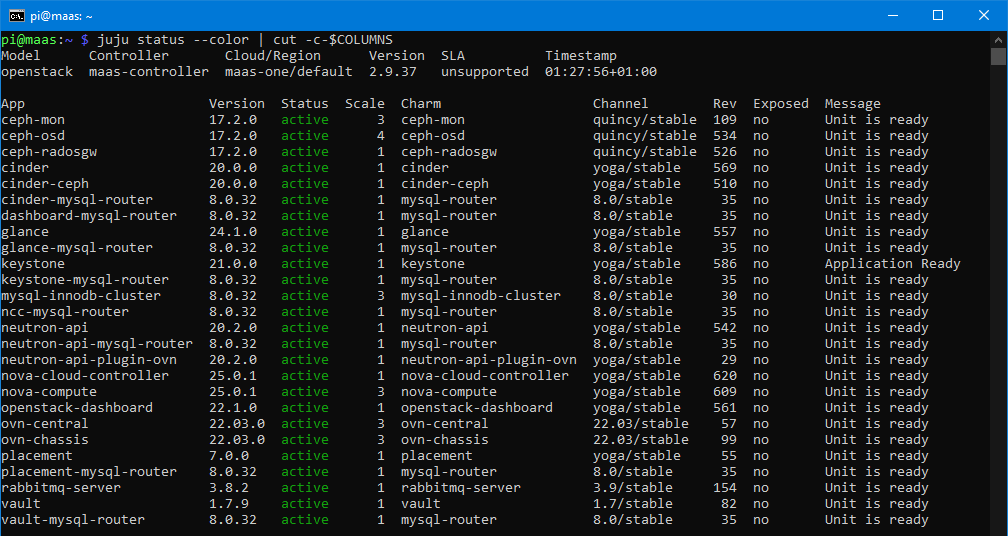
\includegraphics[width=1\linewidth]{tesi/files/immagini/openstack/finish(app).png}
    % \vspace*{-8mm}
    \caption{Status finale del cloud OpenStack post deployment con i charm: elenco delle App (i message sono tagliati per motivi di spazio).}
    \label{fig:juju_status_finish_app}
\end{figure}

\begin{figure}%[H]
    \centering
    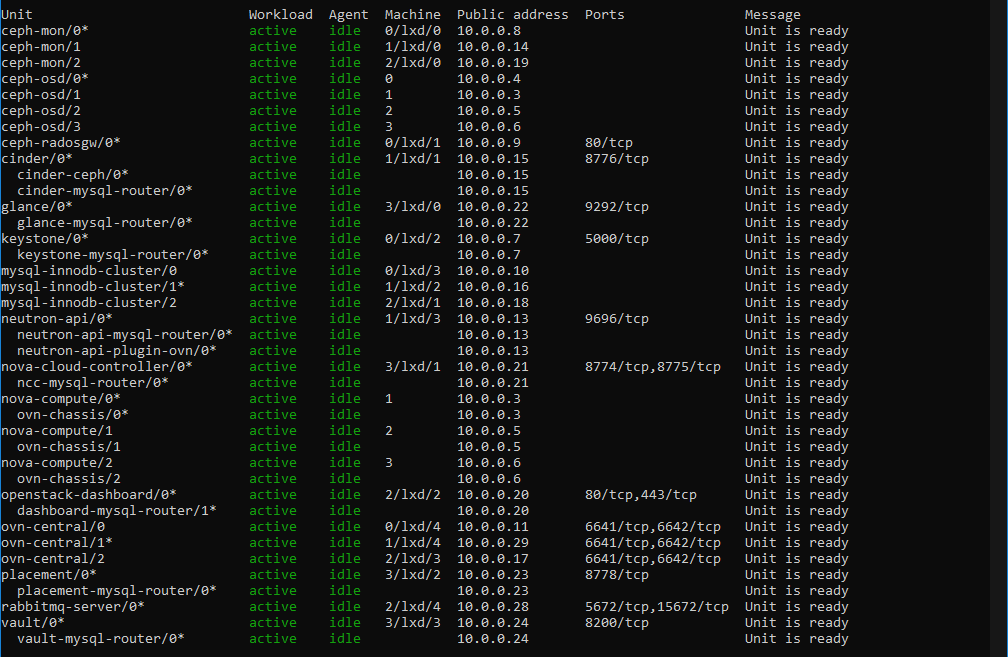
\includegraphics[width=1\linewidth]{tesi/files/immagini/openstack/finish(unit).png}
    % \vspace*{-8mm}
    \caption{Status finale del cloud OpenStack post deployment con i charm: elenco delle Unit (i message sono tagliati per motivi di spazio).}
    \label{fig:juju_status_finish_unit}
\end{figure}

\begin{figure}%[ht]
    \centering
    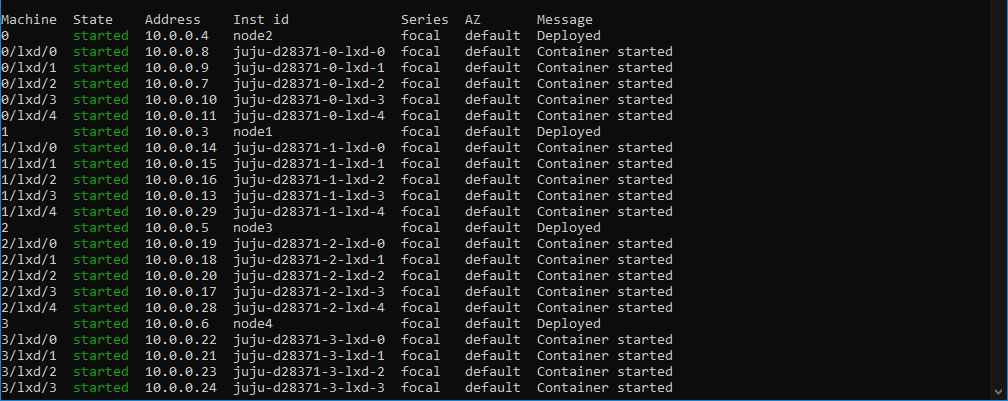
\includegraphics[width=1\linewidth]{tesi/files/immagini/openstack/finish(machine).png}
    % \vspace*{-8mm}
    \caption{Status finale del cloud OpenStack post deployment con i charm elenco delle Machine.}
    \label{fig:juju_status_finish_machine}
\end{figure}



\subsection{Accesso alla dashboard Horizon.}\label{subsec:openstack_dashboard}
Ora è finalmente possibile utilizzare il cloud OpenStack.
% 
Come prima cosa, bisogna ricavare i dati per poter accedere alla dashboard del cloud.
% 
Per ricavare l'indirizzo IP della web app è possibile sia cercarlo manualmente sotto la unit \code{openstack-dashboard/0*} nell'output del comando \code{juju status} (come mostrato in \cref{fig:juju_status_finish_unit}) sia estrapolarlo utilizzando la combinazione di comandi mostrati nel \cref{lst:openstack_install_ip_dashboard}.
% \begin{minipage}{0.96\linewidth} 
\begin{lstlisting}[
    language=mybash, 
   caption={Comandi per estrapolare l'IP della dashboard Horizon. },
    label={lst:openstack_install_ip_dashboard},
]
juju status --format=yaml openstack-dashboard | grep public-address | awk '{print $2}' | head -1
\end{lstlisting}
% \end{minipage}
In questo progetto di testi, l'indirizzo IP che è stato riservato in maniera automatica al charm openstack-dashboard è \code{10.0.0.20}.
 
% \bigskip\noindent
\vspace{1cm}\noindent
Dopodiché, è necessario conoscere le credenziali dell'amministratore di sistema.
% 
La password può essere richiesta a Keystone come mostrato nel seguente listato \cref{lst:openstack_install_credenziali}.
% \begin{minipage}{0.96\linewidth} 
\begin{lstlisting}[
    language=mybash, 
   caption={Richiesta a Keystone della password d'amministratore.},
    label={lst:openstack_install_credenziali},
]
juju run --unit keystone/leader leader-get admin_passwd
\end{lstlisting}
% \end{minipage}

% \begin{figure}[H]
%     \centering
%     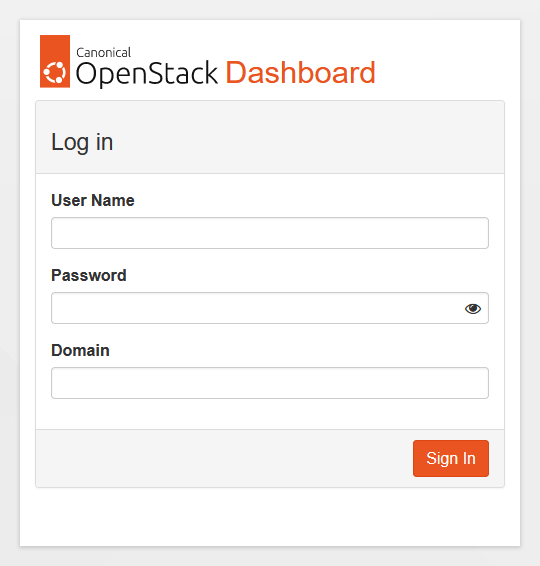
\includegraphics[width=0.7\linewidth]{tesi/files/immagini/openstack/login.png}
%     \caption{Schermata di login della dashboard di OpenStack.}
%     \label{fig:openstack_login}
% \end{figure}

\bigskip\noindent
L'URL della web app a cui collegarsi quindi sarà \code{http://<IP>/horizon/}\\
(o se si volesse usare il protocollo https \code{https://<IP>/horizon/}), in questo caso:
% 
\begin{itemize}
    \item[]URL: \textbf{http://10.0.0.20/horizon/}
\end{itemize}
% 
Una volta collegatosi da qualsiasi browser web
all'indirizzo, apparirà la schermata di log-in come mostrato in \cref{fig:openstack_login}.

\begin{figure}[H]
    \centering
    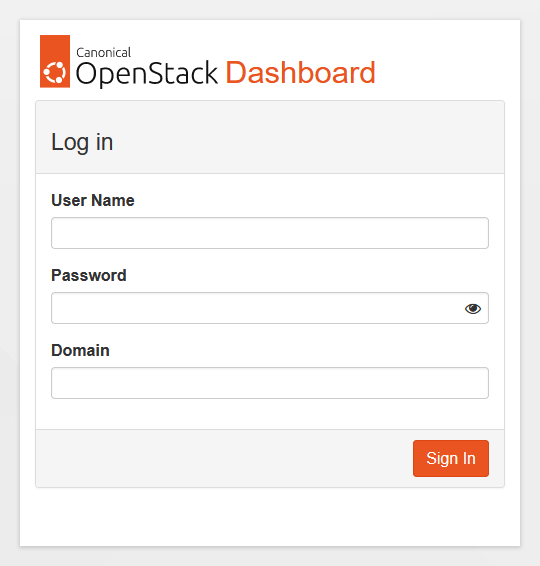
\includegraphics[width=0.5\linewidth]{tesi/files/immagini/openstack/login.png}
    \caption{Schermata di login della dashboard di OpenStack.}
    \label{fig:openstack_login}
\end{figure}

\bigskip
Le credenziali dell'amministratore da immettere sono:
% 
\begin{itemize}
    \item[]Username: \textbf{admin}
    
    \item[]Password: \textbf{ejco3C6Wgxj2je9B}
    
    \item[]Domain: \textbf{admin\_domain}
\end{itemize}

\bigskip\noindent
A log-in effettuato, apparirà la schermata iniziale, da cui poter utilizzare il cloud (\cref{fig:openstack_dashboard}).

\begin{figure}[H]
    \centering
    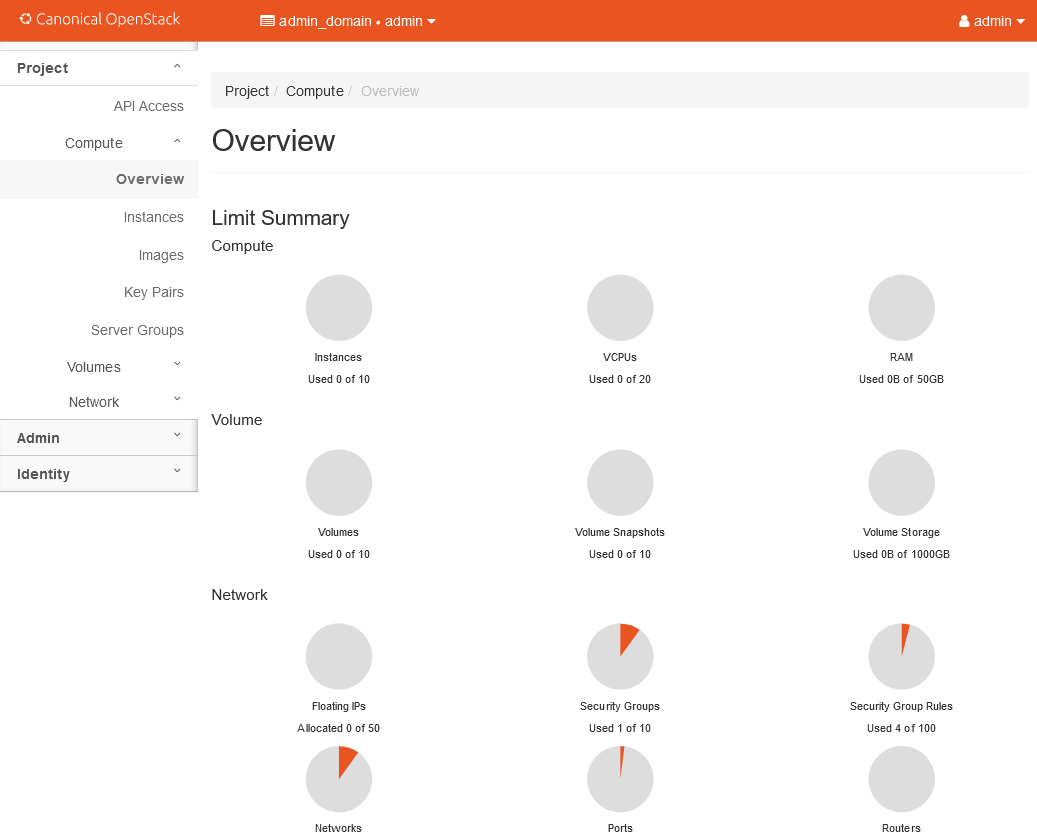
\includegraphics[width=0.95\linewidth]{tesi/files/immagini/openstack/dashboard.png}
    \caption{Schermata post log-in della dashboard di OpenStack con qualche risorsa in uso.}
    \label{fig:openstack_dashboard}
\end{figure}
